\section{Sterowanie}

Do sterowania rotorem wykorzystano możliwości programu Orbitron, który pozwala śledzić ruch satelit poruszających się na orbicie okołoziemskiej. Użytkownik jest w stanie otrzymać informacje o położeniu danego satelity na orbicie oraz wysyłać komunikaty z informacją o kącie azymutu i elewacji anteny jaki należy ustawić, żeby namierzyć wybranego satelitę. Na Rys. \ref{fig:rotor} poniżej zamieszczono widok ekranu głównego aplikacji. 

\begin{figure}[h]
	\centering
		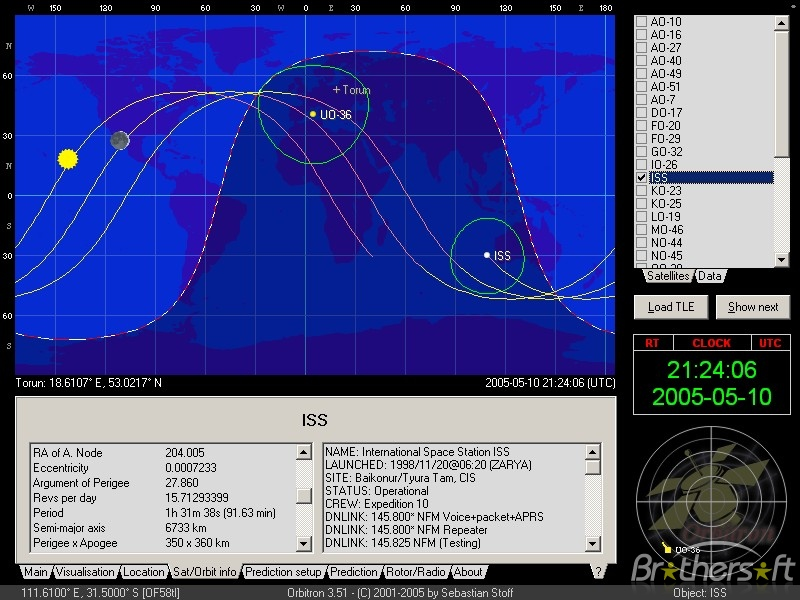
\includegraphics[width=0.7 \textwidth]{orbitron}
	\caption{Widok ekranu głównego programu Orbitron}	
	\label{fig:rotor}
\end{figure}

Aby nawiązać komunikację z układem sterującym rotorami zainstalowano aplikację, będącą dodatkiem do programu Orbitron - \textit{DDE Orbitron To Serial} \cite{dde}. Program na bieżąco może pobierać informacje o położeniu satelit i wysyłajać komunikaty poprzez port szeregowy do układu sterującego rotorem.


\begin{figure}[h]
	\centering
		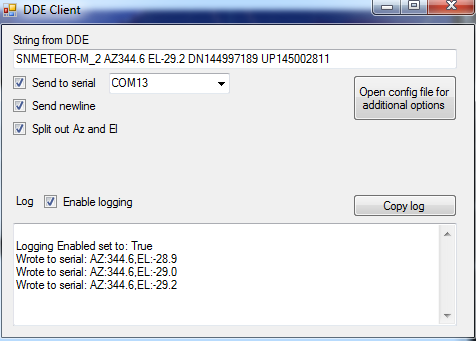
\includegraphics[width=0.7 \textwidth]{DDEOrbitronToSerialScreenShot}
	\caption{Widok okienka aplikacji DDE Orbitron To Serial}	
	\label{fig:rotor}
\end{figure}

Komunikaty z informacją o kącie elewacji i azymutu anteny są wysyłane bezpośrednio do płytki Arduino Uno. Program mikrokontrolera umożliwia sterowanie dwoma silnikami rotora oraz jako sprzężenie zwrotne odbiera dane z enkoderów umieszczonych na osiach silników. Mikrokontroler zlicza impulsy odebrane z czujników co daje pełną informację o rzeczywistym ustawieniu anteny i umożliwia ewentualną korektę. Silniki rotora są silnikami prądu stałego z przekładnią i pozwalają na obrót ze stałą prędkością, więc aby obrócić oś o określony kąt zbadano jaka ilość impulsów enkodera odpowiada pełnemu obrotowi. 
